\begin{problem}{Gyakkyou Burai Kaiji}
{gyakkyou.in}{gyakkyou.out}
{4 seconds}{256 mebibytes}

% Author: Akai, PTZ Summer 2011
% Перевод: Анна Малова

\epigraph
{
%Вы не должны позволять королям как мне ?? % не могу подобрать перевод
You shouldn't let kings like myself draw twice.
}{}

Однажды, прежде чем появится здесь.
Каиджи потерял все.
Единственное, что у него осталось~--- жалкая жизнь.

%\begin{figure}
%{10.5cm}
%{
    \vspace{1em}
    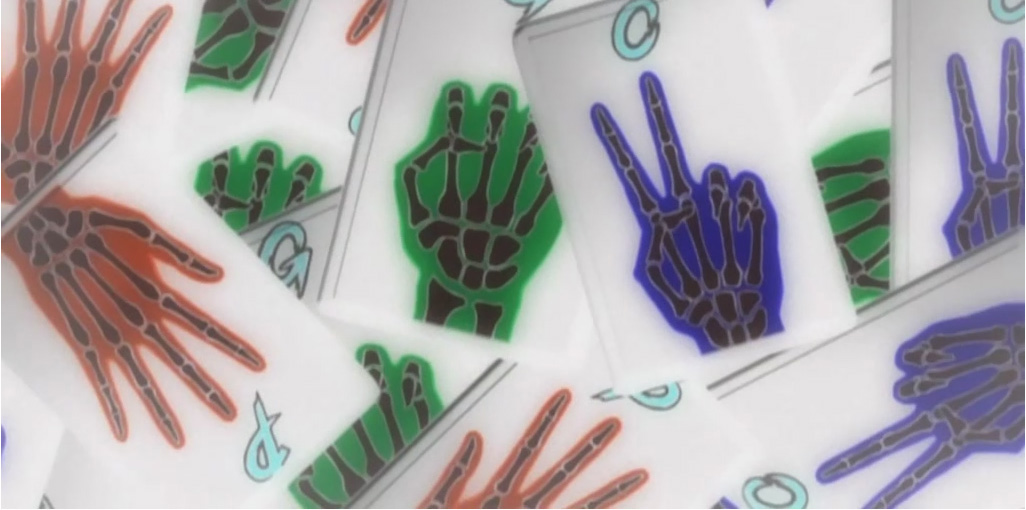
\includegraphics[width=200pt]{pics/g.jpg}
    \vspace{1em}
%}
%\end{figure}

Правила этой игры практически такие же. Есть $N$ различных типов карт, все типы пронумерованы числами от $1$ до $N$ включительно.
Каиджи хранит свои карты в колодах. Карты одинакового типа он кладет в одинаковые колоды, а карты разного типа в разные.
Индекс каждой колоды совпадает с индексом типа карт, которые она содержит.

В любой момент времени, у Каиджи может быть от $0$ до $999\,999\,999$ карт каждого типа.
Однако, сейчас игроки не могут купить, продать или обменяться картами.
Таким образом, количество карт каждого типа, которое есть у Каиджи, остается одинаковым в течение всей игры.
В течение хода, Каиджи может сыграть, используя только одну колоду с индкексами из отрезка $[i, j]$ где $i$ и $j$ параметры хода.

Каиджи уже изучил поведение и стратегии всех игроков и разработал выигрышную стратегию.
Теперь все, что ему надо, это быстро находить ответы к текущему типу вопроса:
на ходе с параметрами $i$ и $j$, какое количество карт в $k$-й по величине колоде среди колод, которые он использует?
Помогите ему ответить на эти вопросы.

Первая строка содержит целое число $N$, количество типов карт ($1 \le N \le 450\,000$).

Вторая строка используется, чтобы сгенерировать целые числа $a_i$, начальное количество карт каждого типа, которое есть у Каиджи
($0 \le a_i < 10^9$). Она содержит три целых числа $a_1$, $l$ и $m$.
($0 \le a_1, l, m < 10^9$);  $2 \le i \le N$,
$$a_i = (a_{i-1} \cdot l + m) \bmod 10^9\text{.}$$


Третья строка содержит целое число $B$~--- число противников ($1 \le B \le 1000$).
$B$ следующих строк описывают множество игр с отдельным противником.
Каждое множество описывается десятью целыми числами.
Первым идет число $G$~--- число игр, сыгранных с этим противником.
Затем следуют $x_1$, $l_x$ и $m_x$, потом $y_1$, $l_y$ и $m_y$,
и наконец, $k_1$, $l_k$ и $m_k$
($1 \le x_1 \le y_1 \le N$, $1 \le k_1 \le y_1 - x_1 + 1$,
$0 \le l_x, m_x, l_y, m_y, l_k, m_k < 10^9$).
Они используются, чтобы сгенерировать вспомогательную последовательность $x_g$ и $y_g$ и
текущие параметры $i_g$, $j_g$ и $k_g$ для $1 \le g \le G$:
$$
\begin{array}{ccll}
x_g & = & ((i_{g - 1} - 1) \cdot l_x + m_x) \bmod N) + 1, & 2 \le g \le G \\
y_g & = & ((j_{g - 1} - 1) \cdot l_y + m_y) \bmod N) + 1, & 2 \le g \le G \\
i_g & = & \min(x_g, y_g), & 1 \le g \le G \\
j_g & = & \max(x_g, y_g), & 1 \le g \le G \\
k_g & = & (((k_{g - 1} - 1) \cdot l_k + m_k) \bmod (j_g - i_g + 1)) + 1,
& 2 \le g \le G \\
\end{array}
$$
Сгенерированные параметры означают, что в $g$-й игре с текущим противником,
Каиджи хочет знать количество карт в $k_g$-й по величине колоде среди всех колод с индексами из отрезка $[i_g, j_g]$.
Общее количество игр, сыгранных Каиджи, не превышает $600\,000$.
\OutputFile

Для каждой игры $g$ с каждым противником $b$, найдите число карт в $k_g$-й по величине колоде,
среди его колод с индексами из отрезка $[i_g, j_g]$.
Выведите одно число: сумму всех этих значений.

\Example

\begin{example}
\exmp{
5
1 1 1
5
1 1 0 0 3 0 0 2 0 0
1 2 0 0 5 0 0 3 0 0
1 1 0 0 5 0 0 5 0 0
1 3 0 0 3 0 0 1 0 0
1 1 0 0 4 0 0 1 0 0
}{
15
}%
\end{example}

\medskip

У Каиджи есть $i$ карт $i$-го типа для всех $i = 1, 2, 3, 4, 5$.
Каждый тип выбирается только один раз.
Таким образом ответ $15$.

\end{problem}
